\begin{figure*}[t]
\centering
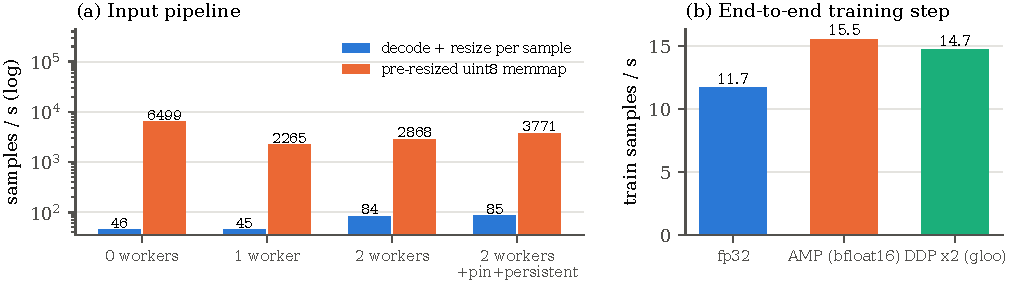
\includegraphics[width=\textwidth]{figures/throughput.pdf}
\caption{Throughput on the 2-core CPU machine used for all experiments. (a) Input pipeline:
decoding and resizing the original radiographs per sample, versus a pre-resized uint8
memory-mapped cache, for several \texttt{DataLoader} settings. (b) One end-to-end training step
of pixel-input IRENE-MM (batch 16), in fp32, with bf16 autocast, and with DDP over 2 Gloo
processes (1 thread each).}
\label{fig:throughput}
\end{figure*}

\Cref{fig:throughput} reports the engineering measurements we could make without a GPU.
Many source radiographs are large JPEG/PNG files, and decoding and resizing them for every
sample limits the input pipeline to \TpDecodeZero{} samples/s in the main process. Two worker
processes help ($\times$\TpWorkerSpeedup{}, \TpDecodeBest{} samples/s). Pre-resizing once into a
memory-mapped uint8 array takes \TpCacheSec{}\,s and raises throughput to \TpMmapBest{}
samples/s ($\times$\TpSpeedup{}). With so little per-sample work on 2 cores, worker processes
then \emph{reduce} throughput because of inter-process transfer. The right
\texttt{num\_workers} depends on the per-sample cost, and should be measured rather than set
by habit. Persistent workers avoid re-forking at every epoch and help consistently when
workers are used. For the model, bf16 autocast raises end-to-end training throughput from
\TpFp{} to \TpAmp{} samples/s on this CPU. DDP with two single-threaded Gloo ranks reaches
\TpDDP{} samples/s, against \TpFp{} for one process with two threads. The same \texttt{train.py}
runs unchanged with NCCL and fp16 loss scaling on GPUs, but we could not measure GPU
utilisation here and make no claim about it.
